\chapter{Introduction and Literature Review}

\section{Introduction}
\label{sec:introduction}

Choreographic programming (CP)
is a language paradigm for implementing distributed systems in which the programmer writes one unified program, called a choreography,
that describes how the participants of the system interact
from a third-person-omniscient perspective.~\shortcite{montesi-carbone-dfbd,montesi-dissertation,montesi_book}
A choreography can be translated into to a collection of executable programs for use in the real world, one for each participant;
this process is called endpoint projection (EPP).
The CP approach has benefits both for understandability of distributed system implementations,
and for strong static guarantees about the deadlock-freedom of the resulting executable code~\cite{montesi-carbone-dfbd}.

The study of CP is comparatively young; while some of the ideas have existed informally as far back as the 1970s,
choreographic programming as it's understood today was first formalized in~\shortcite{montesi-carbone-dfbd}.
In this chapter we describe the central concepts of choreographic programming,
its advantages and disadvantages,
and past and ongoing work to push the boundaries of the kinds of systems it can implement.

\subsection{An illustrative example}

Consider the three programs in \Cref{fig:kvspiecewise},
which are intended to run concurrently and pass messages back and forth between each other.
The overall effect is an elementary process in which the client makes a \inlinecode{Get} or \inlinecode{Put} request to
a server (with a backup) that manages a key-value-store (KVS).
Even this simplified example takes a moment for a reader to make sense of;
one must read the three programs, infer the correspondence between messages sent and received by the three parties,
and judge for oneself if the communication protocol implemented is sensical.
One might even judge that this simple protocol has a bug:
if the request is a \inlinecode{Get}, the backup server will hang indefinitely!

\begin{figure}[tbhp]
  \begin{mdframed}
  \begin{tabular}{c}
  \begin{minipage}{0.95\linewidth}
    \inputminted[xleftmargin=10pt,linenos,fontsize=\scriptsize]{haskell}{figures/kvs_piecewise_client.hs.txt}
  \end{minipage} \\\\
  \begin{minipage}{0.95\linewidth}
	  \textbf{(a)} The function to be called by the client process.
	  They pass in their \inlinecode{Request} object and send it to the server.
	  Then they receive a response from the server and return it.
  \end{minipage}\\\\
  \hline\\
  \begin{minipage}{0.95\linewidth}
    \inputminted[xleftmargin=10pt,linenos,fontsize=\scriptsize]{haskell}{figures/kvs_piecewise_server.hs.txt}
  \end{minipage} \\\\
  \begin{minipage}{0.95\linewidth}
  \textbf{(b)} The function to be called by the primary server.
	  They pass in a reference to their mutable state, and receive a message of type \inlinecode{Request} from the client.
	  In the case of a \inlinecode{Put} request, they forward it to the backup server and check for the backup's acknowledgement.
	  In either case, they process the request against their own mutable state and send the response back to the client.
  \end{minipage}\\\\
  \hline\\
  \begin{minipage}{0.95\linewidth}
    \inputminted[xleftmargin=10pt,linenos,fontsize=\scriptsize]{haskell}{figures/kvs_piecewise_backup.hs.txt}
  \end{minipage} \\\\
  \begin{minipage}{0.95\linewidth}
  \textbf{(c)} The function to be called by the backup server.
	  They pass in a reference to their mutable state, and receive a \inlinecode{Put} message from the primary server.
	  They process it against their mutable state and send back an acknowledgement message to indicate their success.
  \end{minipage}
  \end{tabular}
  \caption{A Simple Concurrent Protocol: a key-value store with a backup server}
  \label{fig:kvspiecewise}
  \end{mdframed}
\end{figure}

In \Cref{sec:history} we will mention some intermediate frameworks that have historically been used to facilitate
writing large and complicated concurrent protocols,
but here we jump ahead to choreographic programming (CP).
\Cref{fig:kvspseudo} shows the same protocol as \Cref{fig:kvspiecewise}, but implemented as a choreography.
In this form there is no cognitive overhead for matching \inlinecode{send} and \inlinecode{recv} operations,
because matching pairs of them are combined into monolithic \inlinecode{comm} operations.
The entire protocol can be read at once in a sensical order.
(The order in which operations are presented in a choreography is not necessarily the order in which they will happen;
the participants are not guaranteed to all start at the same physical time, or to operate at the same speeds.)
Re-writing the example KVS system as a choreography does not immediately solve the issue
of what the backup server should do in the event of a \inlinecode{Get} request,
but it makes the problem detectable by static analysis.
In fact, the choreography in \Cref{fig:kvspseudo} cannot compile in any real CP system
because \inlinecode{"backup"}'s behavior is ambiguous!
\Cref{fig:kvsconclave} shows two variations of how to realize the KVS behavior in Haskell using our \MultiChor library.

\begin{figure}[tbhp]
  \begin{mdframed}
  \begin{tabular}{c}
  \begin{minipage}{0.95\linewidth}
    \inputminted[xleftmargin=10pt,linenos,fontsize=\scriptsize]{haskell}{figures/kvs_pseudo.hs.txt}
  \end{minipage} \\\\
  \begin{minipage}{0.95\linewidth}
	  This pseudo-code choreography implements the protocol from \Cref{fig:kvspiecewise} as a single program.
	  As written, it is not actually realizable because \inlinecode{backup} doesn't know
	  whether to expect a message or not.
	  Real CP systems have ways of detecting and fixing problems like this.
  \end{minipage}
  \end{tabular}
  \caption{A Simple Choreography: a key-value store with a backup server}
  \label{fig:kvspseudo}
  \end{mdframed}
\end{figure}


\begin{figure}[tbhp]
  \begin{mdframed}
  \begin{tabular}{c c}
  \begin{minipage}{9.75cm}
    \inputminted[xleftmargin=10pt,linenos,fontsize=\scriptsize]{haskell}{figures/kvsconclave_a.hs.txt}
  \end{minipage}
  &
  \begin{minipage}{3.75cm}
    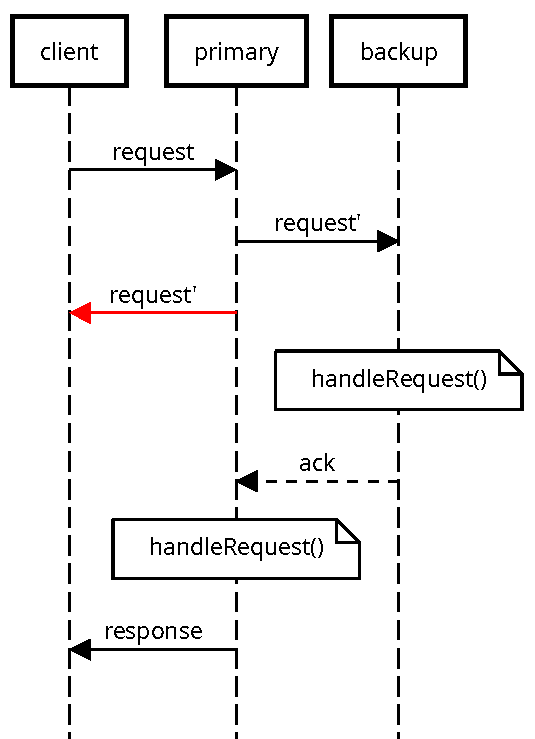
\includegraphics[width=4cm]{figures/seq2.pdf}
  \end{minipage} \\\\
  \multicolumn{2}{c}{\begin{minipage}{0.95\linewidth}
	  \textbf{(a)} A key-value store with a backup server, written in \MultiChor.
           The backup server sends an acknowledgement message \textsf{ack} to the primary server
           if and only if \inlinecode{request} is a \inlinecode{Put}.
           The \inlinecode{broadcast} operator (line 19) ensures KoC
           so that the primary and backup servers are guaranteed to use the same case of \inlinecode{handleBackup},
           but it results in redundant communication (shown in red in the sequence diagram).
  \end{minipage}}\\\\
  \hline\\
  \begin{minipage}{9.75cm}
    \inputminted[xleftmargin=10pt,linenos,fontsize=\scriptsize]{haskell}{figures/kvsconclave_b.hs.txt}
  \end{minipage}
  &
  \begin{minipage}{3.75cm}
     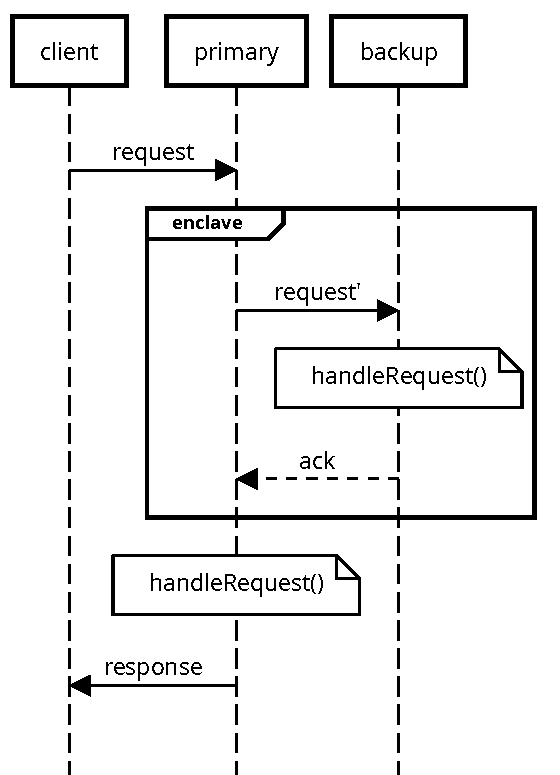
\includegraphics[width=4cm]{figures/seq3.pdf}
  \end{minipage} \\\\
  \multicolumn{2}{c}{\begin{minipage}{0.95\linewidth}
	  \textbf{(b)} In this variation, the \inlinecode{conclave} operator eliminates the redundant communication.
           The conclaved sub-choreography is indicated by a box in the sequence diagram.
           On line~3, \inlinecode{@@ nobody} is \MultiChor idiom explained in \Cref{sec:membership}.
  \end{minipage}}
  \end{tabular}
  \caption{A Real Choreography: a key-value store writing using \MultiChor, two variations.}
  \label{fig:kvsconclave}
    %%\Description{In the top section, twenty four lines of Haskell code using the MultiChor library, with a UML sequence diagram of that program.
%%	The code defines a choreography called "kvs", and helper-functions "handleRequest" and "handleBackup".
%%	In the sequence diagram, first "client" sends "request" to "server",
%%	  then "server" sends "request-prime" to "client" and "backup",
%%	  then backup calls "handleRequest",
%%	  then backup may send "ack" to "server",
%%	  then server calls "handleRequest",
%%	  then server sends "response" to "client.
%%	The bottom sections shows changes to the code in the top section.
%%	In particular, the return type of "handleBackup" is changed to exclude "client".
%%	In the updated sequence diagram, the part of the protocol representing "handleBackup" is in a box named "conclave",
%%	  and the spurious transmission of "request-prime" from "server" to "client" is omitted.
%%	  }
  \end{mdframed}
\end{figure}



\subsection{Layout and Contributions}

The remainder of this chapter covers the history and theory of CP
and discusses some modern work relevant to the ongoing development of CP systems.
In particular, \Cref{sec:knowledge-of-choice} discusses the "Knowledge of Choice" problem,
a central difficulty in the design of CP systems,
and a number of strategies that have been used to solve it.

\Cref{sec:formalism} presents our first contribution:
a formal model of a CP system with
\emph{multiply-located values} (MLVs)
and \emph{conclaves}.
These features combine to allow a compelling new strategy for KoC management.
In particular, all well-typed \HLSCentral choreographies are projectable and have cromulent KoC by construction.
In \Cref{sec:formalism-comparisons} we compare \HLSCentral to representative systems that use other KoC management strategies.

\Cref{sec:multichor} presents our second contribution: an implementation of the conclaves-\&-MLVs paradigm in Haskell.
The \MultiChor library is already available on Hackage, Haskell's main package management system.
\MultiChor directly implements the main concepts of \HLSCentral as a monadic eDSL in Haskell,
and combines Haskell's Hindley–Milner-based type system with a proof-witness system
to capture the requisite notion of a well-typed choreography.

Our third contribution is \emph{census polymorphism},
a design pattern for choreographies that different CP systems may or may not support.
\MultiChor is the first system to support census polymorphism\footnote{
	We do not rule out the possibility that pre-existing systems exist
	in which it might be possible to recapitulate the patterns we describe in this work.
},
by which we mean the ability to write choreographies
that are parametric over their set of participants.
Because \MultiChor is fully embedded in and interoperable with Haskell,
functional-programming patterns can be applied to the choreographic setting without further theoretical or infrastructural work.
\MultiChor's census polymoprhism functions work by applying advanced type-level programming techniques native to mordern Haskell
to \MultiChor's core API.
We discuss census polymorphism in greater detail in \Cref{sec:census-poly}.

\Cref{sec:future} expores possibilites for the future developent of \MultiChor,
including our forth main contribution:
We show that located values are not a necessary primitive component of CP systems
by developing \minichor,
a variant of \MultiChor which can implement the same choreographies using only conclaves, communication, and local computation on normal ("naked") values.
In \Cref{sec:future} we also discus some usability issues with \MultiChor,
and consider how these different findins can apply to future systems.



\section{Background}
\label{sec:background}

Choreographic programming is a paradigm that expresses a distributed system
as a single, global program describing the behavior and interactions of all parties.
The global view of the distributed system enables easier reasoning about the system's behavior;
for example choreographic languages can ensure \emph{deadlock freedom}~\cite{montesi-carbone-dfbd}
and choreographies can be composed modularly like normal single-threaded protocols.

\subsection{History}
\label{sec:history}
Although in this present work we use the noun "choreography" to refer to actual programs written in CP systems,
the word was already in use before the invention of choreographic programming \textit{per se}.
The broader sense of the word is any unified 3rd-person description of or plan for interaction between two or more participating systems.
Pseudo-code diagrams featuring a unified communication operator "→"
were being used to describe cryptographic protocols at least as early as 1978 \cite{needham_schroeder_1978}.
\cite{w3c2005} presented the \emph{"Web Services Choreography Description Language"}
in which a user could specify the interaction, the sequence of communications, between parties.
This was a specification language; implementations compatible with a given specification needed to be written separately.
Later tools were to developed to statically check if a specification was actually implement\emph{able},
whether a provided implementation was faithful to a specification,
and whether the specification had other desired properties.
In particular, \emph{multiparty session types} are a system in which a communication plan is specified as a "global type";
the global type is \emph{projected} to a single party,
resulting in a "local type" against which an implementation of that party's role can type-check
\cite{honda-mpsts}.
Multiparty session types also provided communication safety (\eg a party never misinterprets received data as being of the wrong type)
and a form of deadlock freedom.
One way to think about choreographic programming is as the extension of multiparty session types to include
both the communication plan and the implementation of the computation each party is doing.

For a comparison between choreographic programming and the closely-related field of \emph{multitier langauges}, we refer to~\cite{multiparty-languages}.

\subsection{Endpoint Projection}
\label{sec:endpoint-projection}
CP systems necessarily include a means by which a given computer can execute the behavior of a role in the choreography.
Typically, this takes the form of a function from choreographies to programs in a "local" language
which the target computer can execute.
Such a function is parameterized by the target role, and is called \emph{Endpoint Projection} (EPP);
the roles are "endpoints", \ie surfaces from which and into which messages pass,
and the choreography is "projected" in the sense that the given endpoint's view of it is extracted.

As an example, EPP of the choreography in \Cref{fig:kvsconclave}\emph{(b)} to each of the three participants
would yield respective programs very similar to the ones in \Cref{fig:kvspiecewise},
except that the primary server would always send the request to the backup server
(and therefor the backup server would know how to proceed).

In a choreographic program, many (in some systems, all) values will be \emph{located}:
they will have explicit or implicit metadata indicating their owner.
EPP of a located value to its owner results in the value itself
(typically with the ownership annotation removed),
and EPP to anyone else results in a special placeholder symbol, \eg $\bot$.
The appearance of $\bot$ in a party's projection is not an error,
but attempting to do any semantic evaluation on $\bot$ would be,
so an important correctness property for choreographies is that parties never do that.

\subsection{Knowledge of Choice}
\label{sec:knowledge-of-choice}

Choreographies with conditionals
(\inlinecode{if}-expressions or anything that could be used for conditional control-flow)
introduce
a challenge for endpoint projection:
\emph{some parties might not know which branch to take!}
This challenge is referred to as the \emph{knowledge of choice}  (KoC)~\cite{castagna-knowledge-of-choice} problem.
All choreographic programming languages include a strategy for KoC
that ensures that relevant parties have enough information to play their part in the program.

The pseudo-code in \Cref{fig:kvspseudo} shows a simple instance of this exact problem:
\inlinecode{backup} doesn't know whether to expect a message or not,
because that decision depends on a value (\inlinecode{request'}) that \inlinecode{backup} doesn't have.
\Cref{fig:kvsconclave}\emph{(a)} implements the KoC strategy used by HasChor~\cite{shen-haschor}: the branch guard is broadcast to everyone.
HasChor's authors knew this to be an inefficient (but expedient) solution.
As we show in \Cref{fig:kvsconclave}\emph{(b)}, \MultiChor can do better.

A more traditional approach,
which we refer to as \emph{select-\&-merge},
is to include in one's language a special operator just for communicating KoC.
This operator is called "\inlinecode[bash]{select}"; it sends a statically-declared flag
to the recipient to select which of that party's possible behaviors should be activated.
For example, \Cref{fig:kvs_snm} shows how our KVS choreography might be expressed in a select-\&-merge system.
Under both the centralized semantics and type analysis, \inlinecode[bash]{select} is a no-op!
During EPP, \inlinecode[bash]{select} results in "offer" and "choose" actions at the receiver and sender, respectively.
Because \inlinecode[bash]{select} doesn't affect typing,
in \Cref{fig:kvs_snm} it would not be possible to encode the need for the lines~9 and~12 in Haskell's type system.
Instead, such CP systems enforce KoC requirements in their "merge" operator, which is applied during EPP.
Any party besides the owner of a branch guard will replace the entire conditional expression with the merge of their projections of the branches.
The merge of two "offer" expressions is an offer of the union of the possible continuations;
merges of any other combinations of expressions are only defined when the two expressions are the same.
Thus, if lines~9 and~12 were omitted from \Cref{fig:kvs_snm}, the error would be detected during EPP to \inlinecode{backup}
when the system tried to merge \inlinecode{{}} with
\begin{minted}[xleftmargin=30pt,fontsize=\small]{haskell}
{ request'' <- recv primary;
  success <- handleRequest request'' backupStateRef;
  send success primary  }
\end{minted}
A substantial body of research has explored the soundness select-\&-merge
and its fundamentals, implementation, and extensions
\cite{montesi-carbone-dfbd,core_choreographies,giallorenzo-choral,robust_choreographies}.
That said, HasChor, \MultiChor, ChoRus, and ChoreoTS all do EPP at runtime\cite{batesenclaves},
so using EPP to detect KoC problems would not be a satisfactory solution for them.

\begin{figure}[tbhp]
  \begin{mdframed}
  \begin{tabular}{c}
  \begin{minipage}{0.95\linewidth}
    \inputminted[xleftmargin=10pt,linenos,fontsize=\scriptsize]{haskell}{figures/kvs_snm.hs.txt}
  \end{minipage} \\\\
  \begin{minipage}{0.95\linewidth}
	  This pseudo-code choreography implements the protocol from \Cref{fig:kvsconclave}\emph{(b)}
	  using "select-\&-merge" syntax.
	  Attempting to engineer a real select-\&-merge CP eDSL in the style of \MultiChor
	  would result in a system that could not detect KoC errors until runtime.
  \end{minipage}
  \end{tabular}
  \caption{A Select-\&-Merge Choreography: a key-value store with a backup server}
  \label{fig:kvs_snm}
  \end{mdframed}
\end{figure}

Yet another KoC strategy was proposed by \cite{jongmans2022predicates}.
Their approach requires writing distinct guards for every
participant in a conditional expression; they show how to use predicate transformers to check that
such distributed decisions are unanimous.
This system is verbose, but at least as expressive as the one we describe in this work.

\subsection{The "Census" typing context}
\label{sec:census}
Although it is a hallmark of CP that a user may write actions for various parties in any given place in the program
without demarcations of who "control" is passing to,
it is not necessarily the case that every party that exists is eligible to take action at every place in the choreography.
Some earlier works, \eg \cite{chor-lambda}, have tracked these sets of participants in their type systems,
and used that typing context to control participation inside of function bodies.
Such a typing context plays a more active role in this present work, so we coin the term \emph{"census"}
for a typing context that controls which parties are "present" to participate in any given part of a choreography.

A party not listed in a census should will typically skip evaluating that section of the choreography.
In terms of EPP, that's done by projecting the entire clause to ⊥ or some similar marker.

\subsection{Additional Literature}
\label{sec:modern-work}

Research and development of CP systems seems to have accelerated since approximately 2022.
Pirouette~\cite{hirsch2021pirouette}, Chorλ~\cite{chor-lambda},
and  PolyChorλ~\cite{graversen2023polychor}
are (higher order) functional languages for writing select-\&-merge choreographies;
PolChorλ additionally introduces polymorphism over identities of parties.
Choral~\cite{giallorenzo-choral} is a choreographic language implementing the select-\&-merge paradigm
and targeting industrial use;
it runs on the JVM and can easily import local Java code.
Dyno~\cite{zakhour23} is a CP system for Android development;
it's key feature is the ability to resolve the location and ownership of data and computation dynamically,
while still providing static safety guarantees.

Excitingly, CP libraries for a variety of general purpose languages have recently appeared on the scene.
These include UniChorn~\cite{unichorn}, Chorex~\cite{chorex-github}, and Klor~\cite{klor-github}.
All three are under development; here we report on their state toward the end of 2024.
UniChorn is a port of HasChor into the Unison programming language.
To implement EPP, it uses the Unison feature of \emph{abilities}, better known in the literature as algebraic effects~\cite{plotkin-2003,plotkin-2013}.
This implementation approach, which was also recently proposed by~\cite{shen-alg-eff-cp},
can be thought of as a generalization of the free(r)-monad approach.
As a direct port of HasChor, UniChorn does not support conclaves, MLVs, or census polymorphism.
Chorex is a CP system for Elixir, and Klor is a CP system for Clojure;
both Chorex and Klor leverage the powerful macro systems of their respective host languages to carry out EPP.
Chorex uses the select-\&-merge KoC strategy, and unprojectable choreographies can be detected at macro expansion time.
Klor, on the other hand, is effectively an conclaves-\&-MLVs system, but their API differs from the implementations we present here,
and the authors have not yet shown what safety guarantees it does or does not offer.
Neither Chorex nor Klor support census polymorphism.

Wysteria~\cite{wysteria} and Symphony~\cite{Sweet_2023} are domain-specific languages for \emph{secure multiparty computation}.
Programs in these languages can exhibit census polymorphism,
but they have homomorphic encryption baked into their
semantics for communication,
and they are not intended for general-purpose choreographic programming.
Wysteria has a \inlinecode{par} language construct, used for evaluating an expression at a set of locations,
that is somewhat similar in spirit to our conclaves.
However, applying the conclave concept to choreographic programming, and to the choreographic knowledge-of-choice problem in particular,
is to our knowledge a novel contribution of this paper.
Symphony does not support conditionals, and therefore KoC propagation is a moot point for them.



\bibliographystyle{chicago}
\bibliography{refs}
